\section{Visualization of Time-Oriented Data}
Time is an essential aspect of life; everything contains inherent temporal attributes such as the time when a person was born and the time when an event happens. Long before computers were invented, information graphics have been used to represent temporal relationship of data. One of the oldest documented timelines was created back in 1765 entitled \emph{Chart of Biography} by Joseph Priestley (\autoref{fig:lr-biography-chart}). It shows the lifespans of two thousand famous names along a horizontal time axis, spanning from 1200 BC to 1800 AD. He uses a horizontal line segment to depict a lifespan, and adds dots to either ends to indicate the uncertainty of the reported values. 

\begin{figure}[!htb]
	\centering
	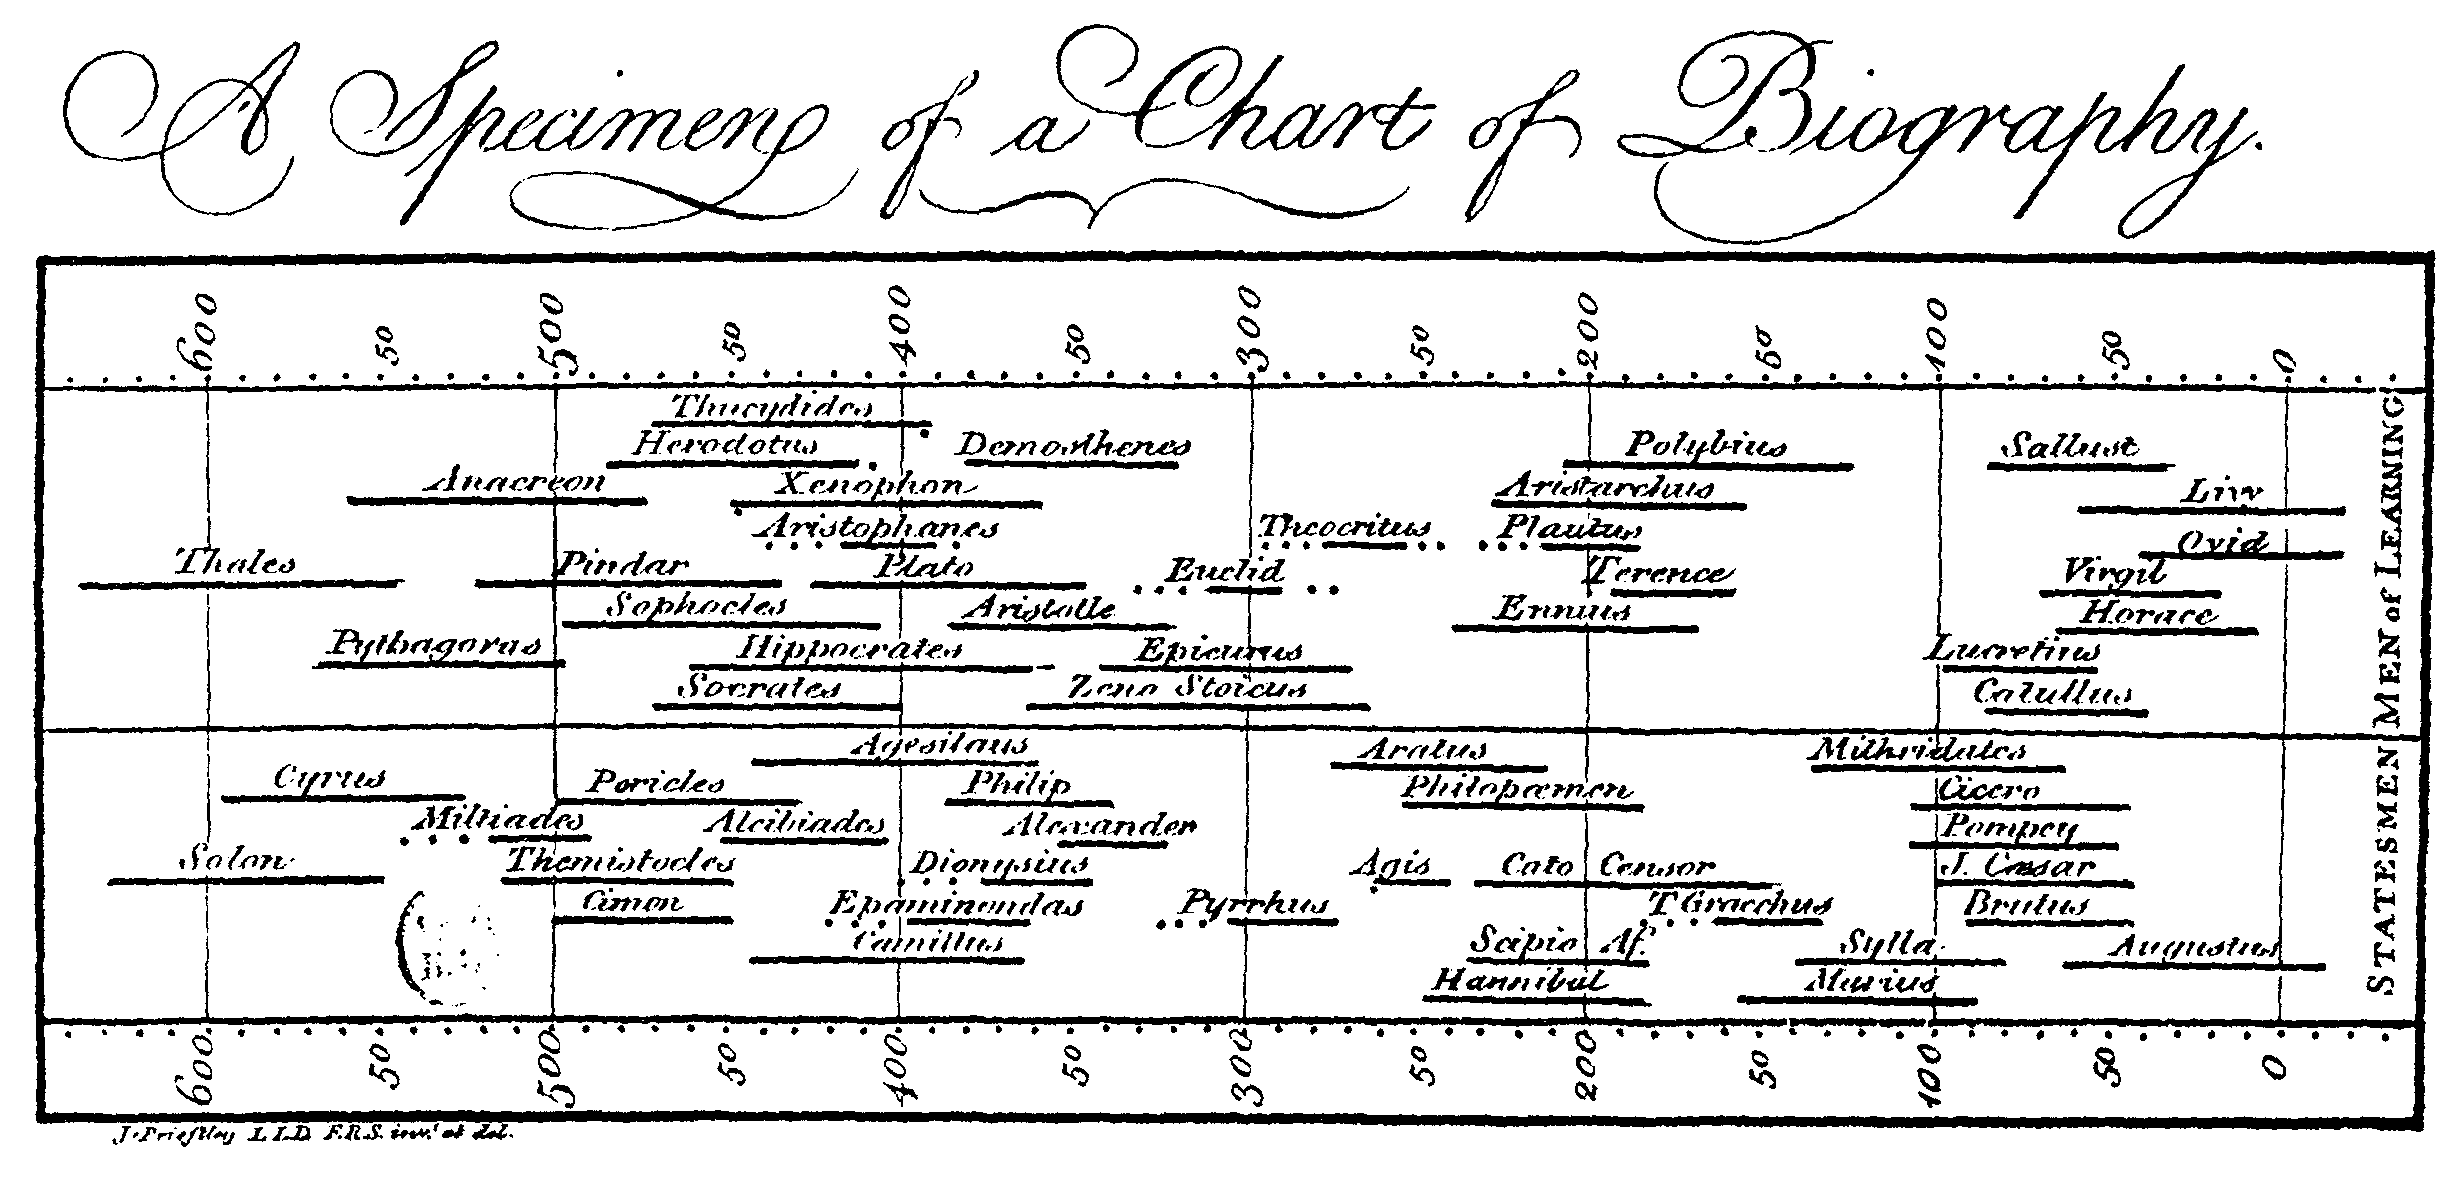
\includegraphics[width=\columnwidth]{biography-chart}
	\caption{Joseph Priestley's Chart of Biography portraying the lifespans of famous historical persons. \is{Priestley1765}}
	\label{fig:lr-biography-chart}
\end{figure}

Since then, many visualization techniques have been developed to effectively reveal the temporal relationship of data. The book by Aigner~et~al.~\cite{Aigner2011} provides a comprehensive review of this topic. In this section, we focus on different visual mappings of time.

\subsection{Horizontal}
The most common representation of time is mapping it to a horizontal axis as in the aforementioned \emph{Chart of Biography}. Data items are positioned along the axis as either a point mark for point-based time or a line mark for interval-based time. Given a two-dimensional space, the vertical axis is available for encoding additional information.

\subsubsection{Scaled Vertical Axis}
Time-series data is a sequence of data points collected at uniform intervals such as population of a country for every year and stock market value for every hour. A time-dependent variable in time-series data is often mapped to a vertical axis. Classic charts such as scatter plot, line chart and bar chart and are all commonly used for this purpose. Scatter plot shows each data point as a point mark, with the x-coordinate mapping to the temporal value and the y-coordinate mapping to the value of the time-dependent variable. Line chart further connects these data points to form a line. Bar chart also shows data points individually like scatter plot, but each data point is represented by a bar, with its height corresponding to its time-dependent value. Line chart is suitable for showing trends of the series, whereas scatter plot and bar chart are good at emphasizing individual data points. With the advantage of visual alignment, bar chart is more effective than scatter plot at comparison of time-dependent values~\cite{Aigner2011}. \autoref{fig:lr-scatter-line-bar} shows an example for each of these three charts.

\begin{figure}[!htb]
\centering
\subcaptionbox{Scatter plot: showing data points as dots. \label{fig:lr-scatter}}{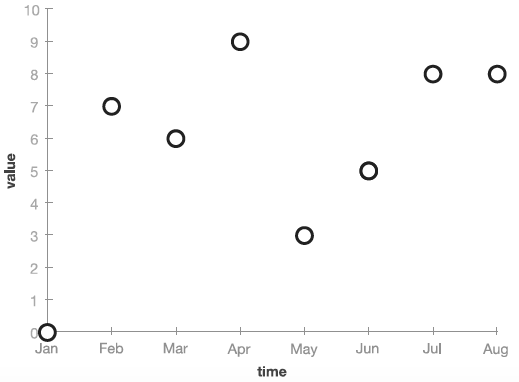
\includegraphics[height=.222\columnwidth]{scatter-plot}}
\hfill
\subcaptionbox{Line chart: connecting data points with lines. \label{fig:lr-line}}{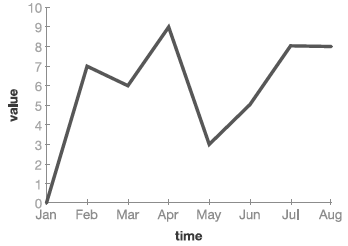
\includegraphics[height=.222\columnwidth]{line-chart}}
\hfill
\subcaptionbox{Bar chart: showing data points as aligned bars. \label{fig:lr-bar}}{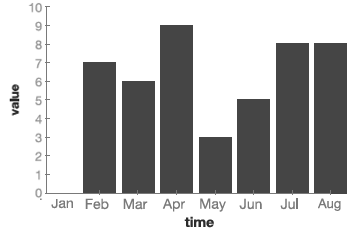
\includegraphics[height=.222\columnwidth]{bar-chart}}
\caption{Three charts showing the same time-series dataset with the horizontal axis representing time and the vertical axis representing a numerical value.}
\label{fig:lr-scatter-line-bar}
\end{figure}

Horizon graph~\cite{Reijner2008} is a recent improvement of line chart for visualizing time-series data, designed for a more space-efficient representation in order to facilitate comparison of different series, such as daily prices for one year of multiple stocks. To make a fair comparison, it shows a derived percentage changes from the earliest data point instead of raw values. Starting from a line chart, the value range is divided into equal bands, such as 10\% for each band, and color coded using a diverging colormap for positive/negative values with increasing color intensity for greater band values. The colored bands allow more precise value reading. Then, the negative values are mirrored into the positive side, reduced the chart height by half. To save more space, those bands are layered with increasing values atop using the two-tone pseudo coloring technique~\cite{Saito2005}. \autoref{fig:lr-horizon-step} illustrates these steps, and \autoref{fig:lr-horizon} shows prices of 50 stocks over a year.

\begin{figure}[!htb]
\centering
\subcaptionbox{The construction steps: color $\rightarrow$ mirror $\rightarrow$ layer. \label{fig:lr-horizon-step}}[.36\columnwidth]{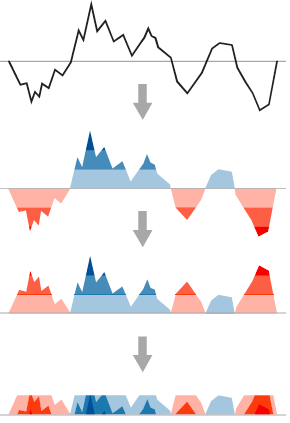
\includegraphics[height=.36\columnwidth]{horizon-graph-step}}
\hfill
\subcaptionbox{A horizon graph showing prices of 50 stocks over a year, each row for a stock. \label{fig:lr-horizon}}{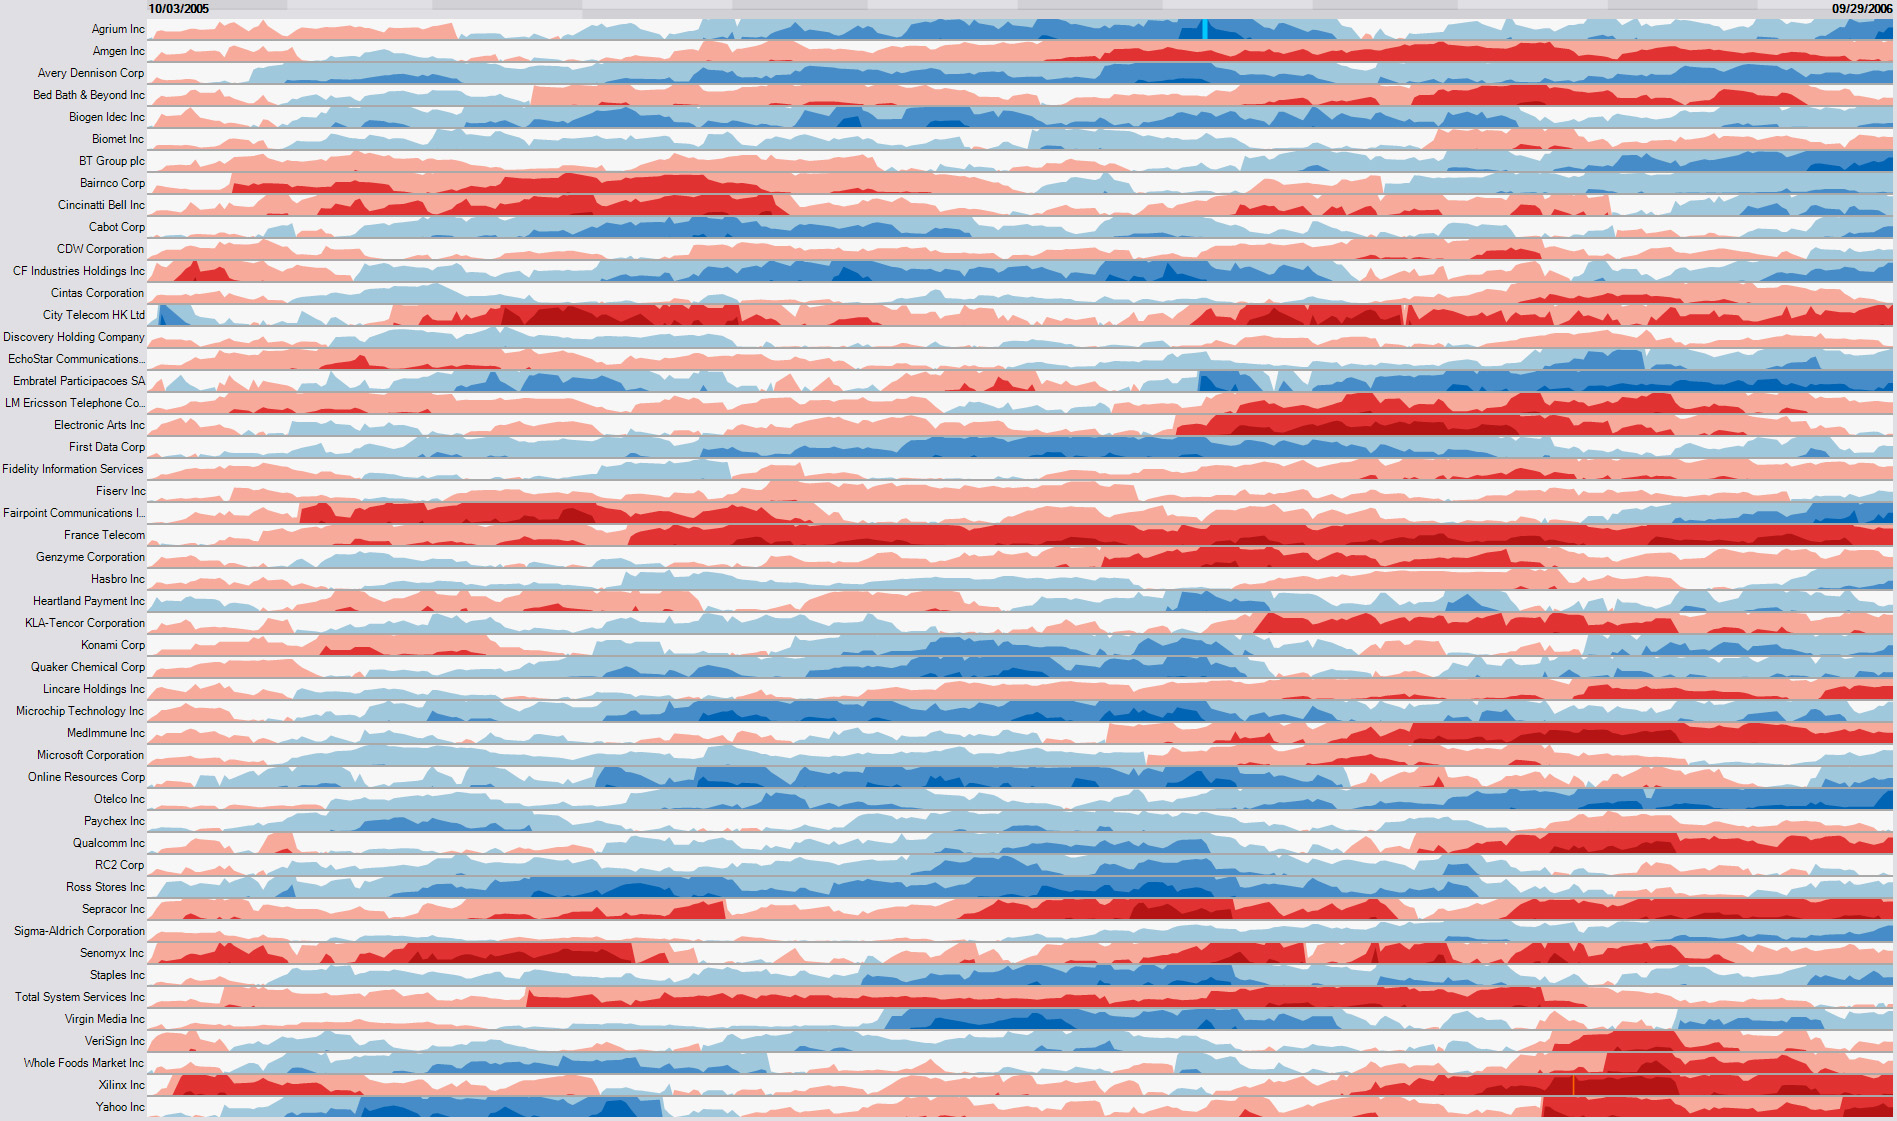
\includegraphics[height=.36\columnwidth]{horizon-graph}}
\caption{Horizon Graph: a space-efficient visualization of time-series data. \is{Reijner2008}}
\label{fig:lr-horizon-graph}
\end{figure}

Horizon graph uses space more efficiently than line chart in visualizing time-series data. A study by Heer, Kong and Agrawala~\cite{Heer2009a} investigates their performances in value comparison tasks. The results show that mirroring a chart (flipping negative values) does not have negative effects; it neither slowed completion time nor hurt accuracy. Moreover, for charts with small sizes, layered bands are even more effective than line chart.

Stacking multiple area charts on top of each other is a suitable approach to visualize multiple time-dependent variables. ThemeRiver~\cite{Havre2002} can be considered as a smooth and symmetric version of stacked graph, designed to show thematic variations over time within a large collection of documents. Each theme is displayed as a colored current flowing through the time, and at any point, the width of the current maps to the strength of the associated theme. The overall river consists of multiple colored currents, providing a good overview of the themes that were important at certain points in time. 

\begin{figure}[!htb]
	\centering
	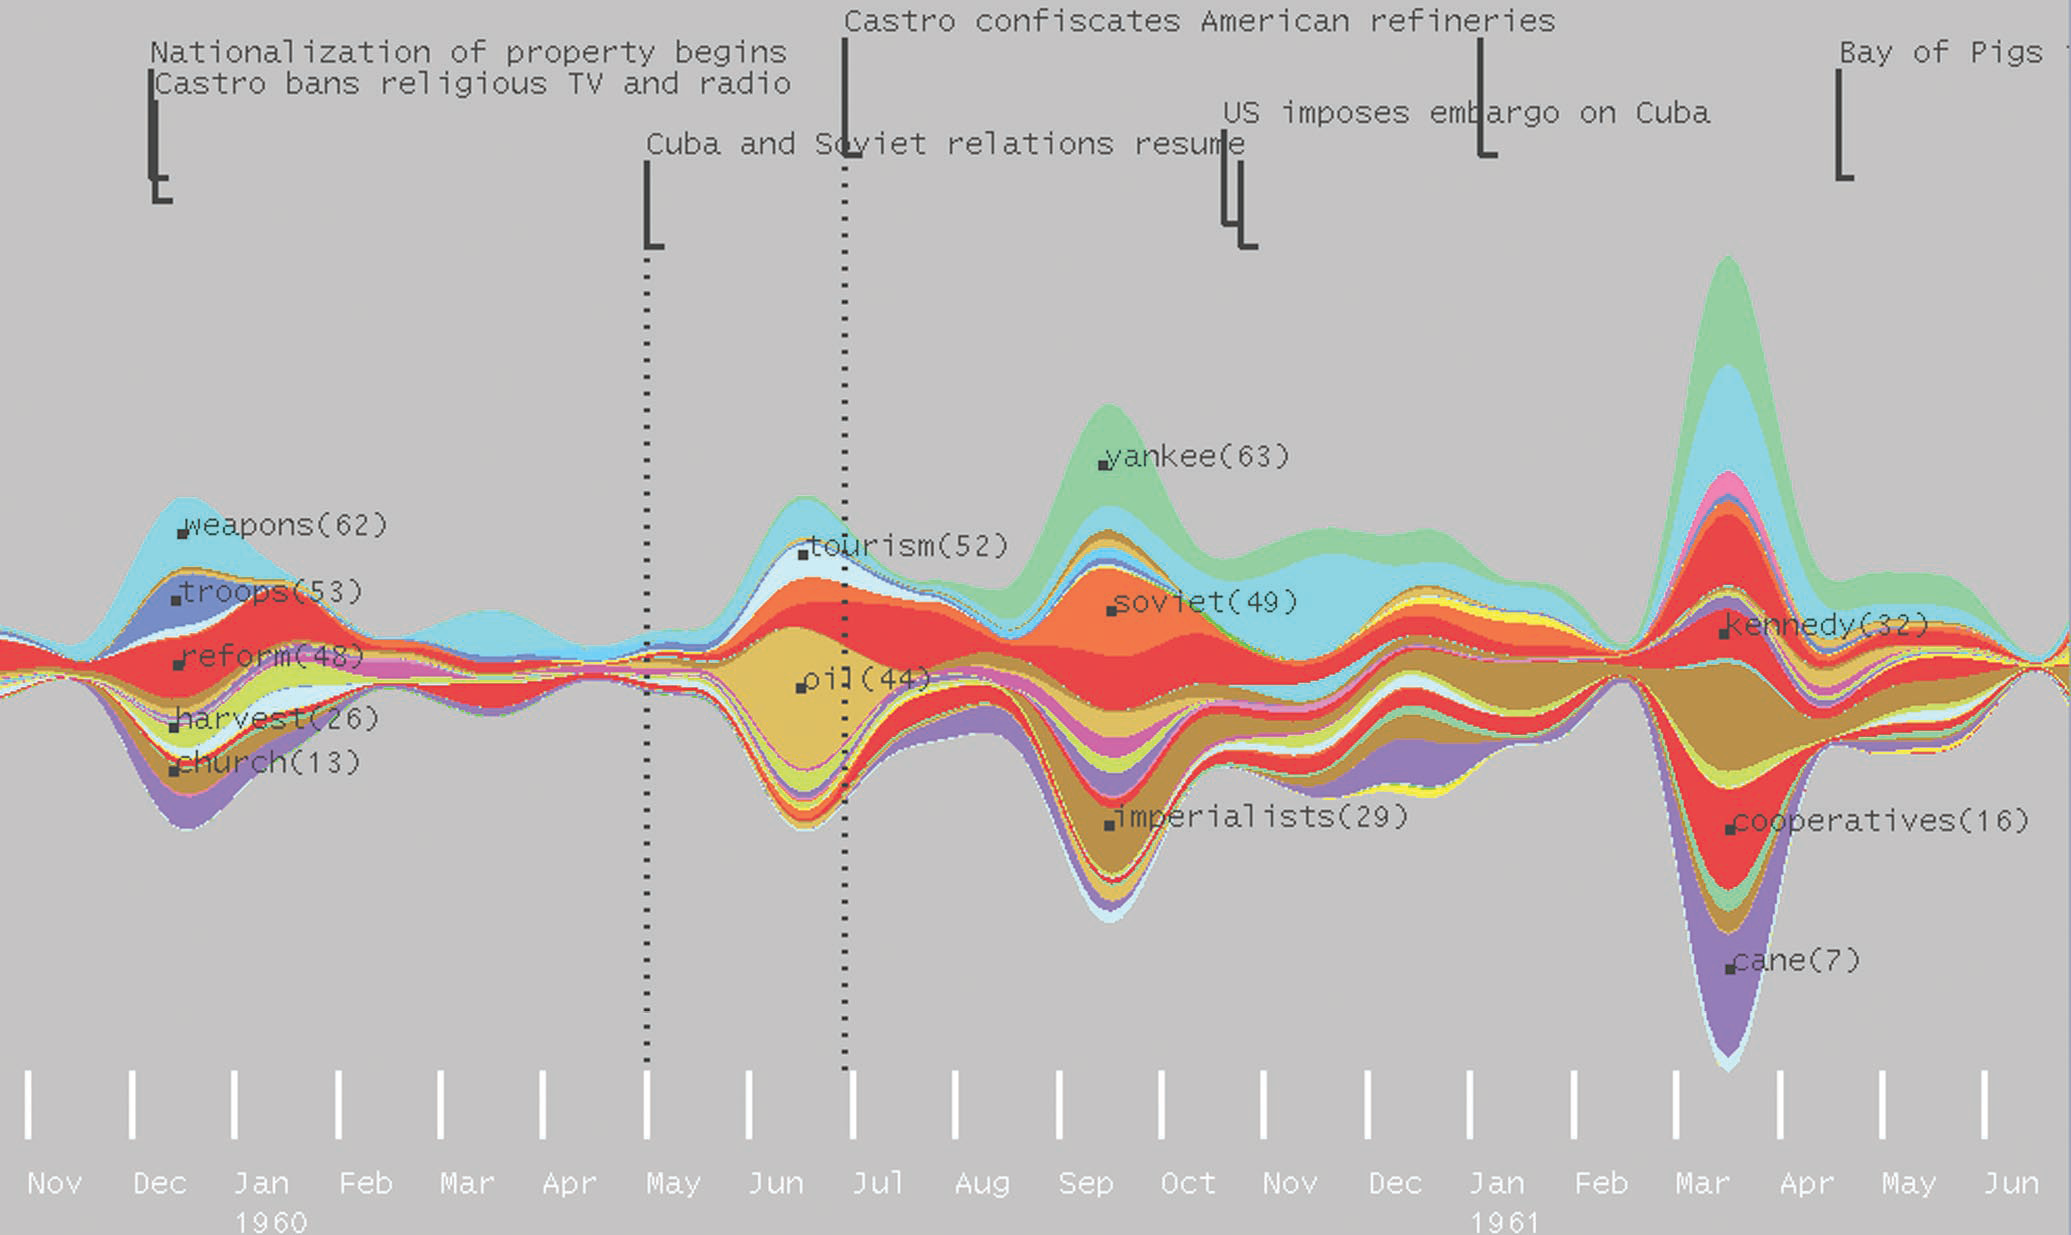
\includegraphics[width=\columnwidth]{theme-river}
	\caption{ThemeRiver uses a river metaphor to represent themes in a collection of Fidel Castro's speeches, interviews and articles from the end of 1959 to mid-1961. Each colored current corresponds a theme. \is{Havre2002}}
	\label{fig:lr-theme-river}
\end{figure}

Byron and Wattenberg discuss considerations of aesthetics and legibility for designing such stacked graphs. \autoref{fig:lr-streamgraph-1} shows the traditional stacked area chart, where the bottom of the lowest layer is a horizontal line at 0. \autoref{fig:lr-streamgraph-2} shows the ThemeRiver version, which is optimized for the symmetry of the entire layout. \autoref{fig:lr-streamgraph-3} shows the Stream Graph~\cite{Byron2008} version, which minimizes the number of wiggles of layers.

\begin{figure}[!htb]
\centering
\subcaptionbox{Traditional stacked graph. \label{fig:lr-streamgraph-1}}{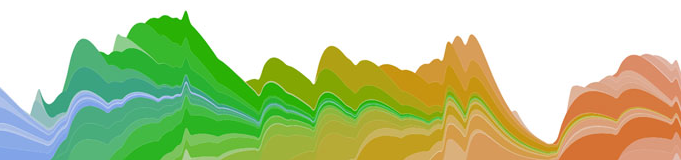
\includegraphics[width=\columnwidth]{streamgraph-1}}

\vspace{0.5cm}

\subcaptionbox{ThemeRiver. \label{fig:lr-streamgraph-2}}{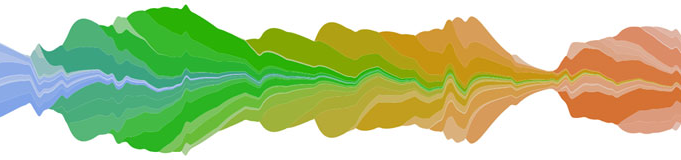
\includegraphics[width=\columnwidth]{streamgraph-2}}

\vspace{0.5cm}

\subcaptionbox{Stream Graph. \label{fig:lr-streamgraph-3}}{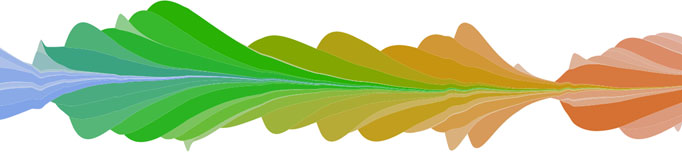
\includegraphics[width=\columnwidth]{streamgraph-3}}
\caption{Stacked graphs with different design considerations. \is{Aigner2011}}
\label{fig:lr-streamgraph}
\end{figure}

\subsubsection{Non-Scaled Vertical Axis}
The vertical dimension may be used to avoid clutter in producing a compact layout. LifeLines~\cite{Plaisant1996,Plaisant1998}, a visualization system of patient records, is a good example. It groups these records into different facets such as problems, allergies, diagnosis and medications, and vertically stack them on top of each other. Within each facet, interval-based records are represented as horizontal bars covering their timespans. Because their timespans may overlap, the layout adjusts their vertical coordinates to avoid intersection. \autoref{fig:lr-lifelines} shows an example of LifeLines. 

\begin{figure}[!htb]
	\centering
	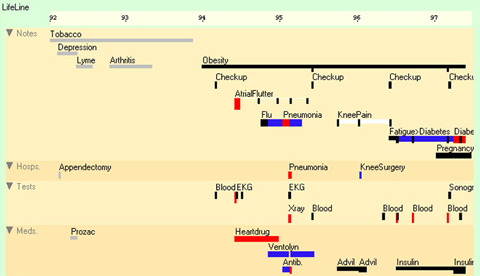
\includegraphics[width=\columnwidth]{lifelines}
	\caption{LifeLines. The timeline consists of several facets, stacked vertically. Each facet includes health-related records shown as horizontal bars, which may be located in different rows to avoid overlapping. \is{Plaisant1998}}
	\label{fig:lr-lifelines}
\end{figure}

Another example is Continuum~\cite{Andre2007}, a timeline visualization of hierarchically structured temporal data such as the relationship of era, composers and pieces. The timeline shows the lifespans of composers as rectangles, where the width represents temporal information, and the height depends on the number of pieces they composed. It also uses vertical position to produce an overlap-free layout.

Temporal visualization often encode additional relationships of data items. Gantt chart~\cite{Gantt1913} is a classic method for displaying planning activities in project management. Each activity is shown as a horizontal bar covering the planning time, and text from the left part of the chart shows activity names. Dependency is a common relationship in planning and can be shown as an arrow. For instance, an arrow pointing from the end of activity $A$ to the beginning of activity $B$ can indicate that $B$ must happen after $A$. Activities are often organized in hierarchical structure such as tasks and sub-tasks. They can be ordered and arranged with indentation to reflect this structure. Timeline tree~\cite{Burch2008} draws an explicit node-link tree on the left part of the timeline to show the hierarchy. \autoref{fig:lr-ganttchart} shows a Gantt chart with hierarchically structured tasks.

\begin{figure}[!htb]
	\centering
	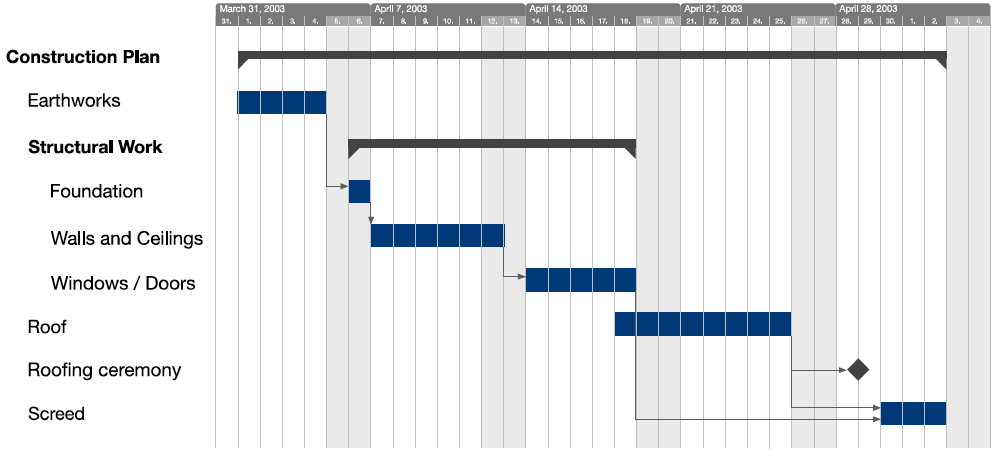
\includegraphics[width=\columnwidth]{gantt-chart}
	\caption{Gantt chart. Each task is shown in an individual row with task name on the left and horizontal bar on the right spanning task time. Arrows show dependency, and label indentation indicates the hierarchy of tasks. \is{Aigner2011}}
	\label{fig:lr-ganttchart}
\end{figure}

Spatial proximity is another method to represent relationships. This method is applied in storyline visualizations to illustrate the dynamic relationships between characters in a movie, which was first introduced by Munroe with his hand-drawn charts~\cite{Munroe2009}. The visualization depicts each character as a curved line and each scene as a bundle of those character lines. Ideally, all the lines within a scene should be horizontally parallel. A line diverges from its bundle if the character leaves the scene, and conversely, a line converges into a bundle if the character joins that scene. Algorithms have been introduced to automate the drawing process, including work by Tanahashi and Ma~\cite{Tanahashi2012} and Liu~et~al.~\cite{Liu2013}. \autoref{fig:lr-storyline} shows the storyline visualization of the \emph{Star Wars} movie.

\begin{figure}[!htb]
	\centering
	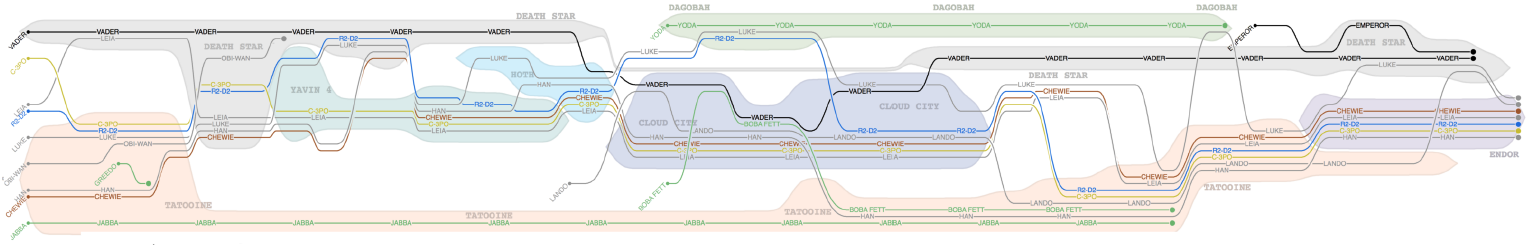
\includegraphics[width=\columnwidth]{storyline}
	\caption{Storyline visualization of the movie \emph{Star Wars}. Each line represents a character, and a bundle of lines represents an interaction of those characters. \is{Tanahashi2012}}
	\label{fig:lr-storyline}
\end{figure}

Similarly, TimeNets~\cite{Kim2010} also applies \emph{proximity} to visualize relationships of genealogical data. It uses a curved line to represent the lifespan of a person. These lines are located spatially distant if the persons they represent are unrelated. Two lines converge if the represented persons marry and diverge when they divorce. Child lines stay close to their parent lines, and dotted vertical lines are drawn from the parents to the beginning of their child lines to indicate the parent-child relationship. \autoref{fig:lr-timenets} shows a TimeNets example depicting these relationships.

\begin{figure}[!htb]
	\centering
	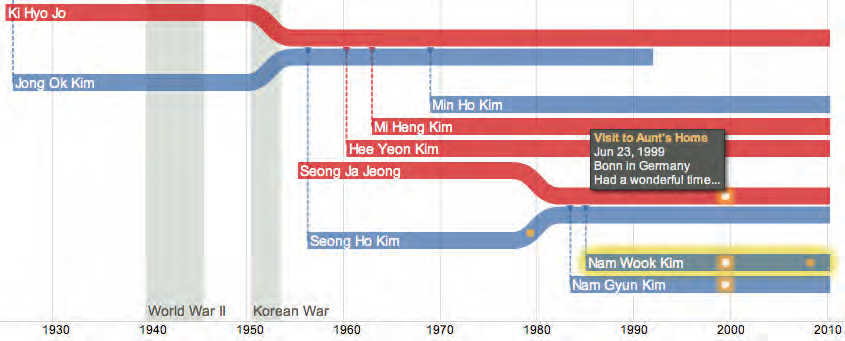
\includegraphics[width=\columnwidth]{timenets}
	\caption{TimeNet visualization of genealogical data. Lifelines represent people, converging lines signify marriage, and drop lines indicate children. \is{Kim2010}}
	\label{fig:lr-timenets}
\end{figure}

\subsection{Spiral}
Another representation of time is mapping it to a \emph{spiral} axis, and data items are positioned along that spiral~\cite{Weber2001}. Color intensity and line thickness are suitable for encoding an additional quantitative variable. For interval-based data, filled curved segments are aligned with the spiral to indicate the two ends of intervals~\cite{Carlis1998}. Spirals can also be intertwined to show multiple variables. \autoref{fig:lr-spiral} shows a spiral graph comparing two variables over time with different color hues. 

\begin{figure}[!htb]
	\centering
	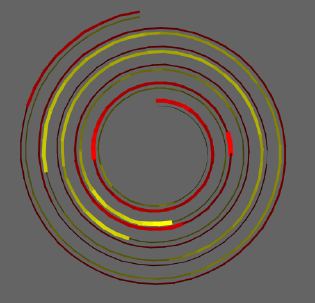
\includegraphics[width=.4\columnwidth]{spiral}
	\caption{Spiral graph. Time is represented along a spiral with color intensity and line thickness are used to indicate time-dependent, numerical values. Two variables are distinguished using different color hue: yellow and red. \is{Weber2001}}
	\label{fig:lr-spiral}
\end{figure}

Spiral graph is effective at spotting periodic patterns of the data, but it highly depends on the cycle length; i.e., the number of time steps per cycle. \autoref{fig:lr-spiral-all} shows three charts using the same time-series dataset. \autoref{fig:lr-spiral-1} uses a bar chart and clearly reveals trends and extreme values. The other two charts use spiral graphs; however, a cyclic pattern is only visible in \autoref{fig:lr-spiral-3}. The difference between them is the cycle length: 24 days for \autoref{fig:lr-spiral-2} but 28 days for \autoref{fig:lr-spiral-3}, which clearly shows a pattern of four weeks. This pattern can also be revealed if the cycle length is set to a small multiple of 7 days. Interaction has been proposed to facilitate users in identifying the right cycle length~\cite{Weber2001,Tominski2008}. Users can manually adjust the cycle length. Alternatively, users can watch an animation of the visualization through different cycle lengths and stop the animation when they find the pattern of interest.

\begin{figure}[!htb]
\centering
\subcaptionbox{Bar chart: revealing trends and extreme values. \label{fig:lr-spiral-1}}{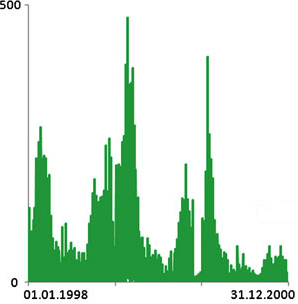
\includegraphics[height=.325\columnwidth]{spiral-1}}
\hfill
\subcaptionbox{Line chart: connecting data points with lines. \label{fig:lr-spiral-2}}{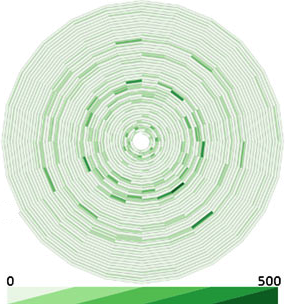
\includegraphics[height=.325\columnwidth]{spiral-2}}
\hfill
\subcaptionbox{Bar chart: showing data points as aligned bars. \label{fig:lr-spiral-3}}{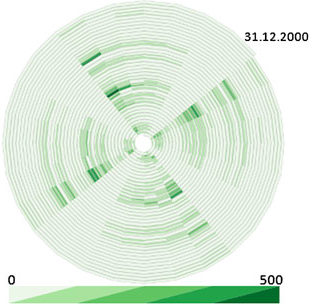
\includegraphics[height=.325\columnwidth]{spiral-3}}
\caption{Different insights can be gained from visual representations depending on whether the linear or cyclic character of the data is emphasized. \is{Aigner2011}}
\label{fig:lr-spiral-all}
\end{figure}

\subsection{Circle}
Time can also be represented using a \emph{tree-ring} metaphor. In a tree, a new layer of wood cells is produced every year, growing out from the center (\autoref{fig:lr-circle-view-1}). Inspired from this phenomenon, Keim, Schneidewind and Sips~\cite{Keim2004} introduce Circle View -- an approach to visualize time-related multidimensional datasets. It splits a circle into multiple concentric rings, each for a time step. The circle is divided into a number of segments, each representing a variable. \autoref{fig:lr-circle-view-2} shows such a view with six variables. Color is used to show the (aggregated) data value for the corresponding interval.

\begin{figure}[!htb]
\centering
\subcaptionbox{Cross section of Douglas Fir tree showing almost perfect  tree-rings. \is{Theron2006} \label{fig:lr-circle-view-1}}{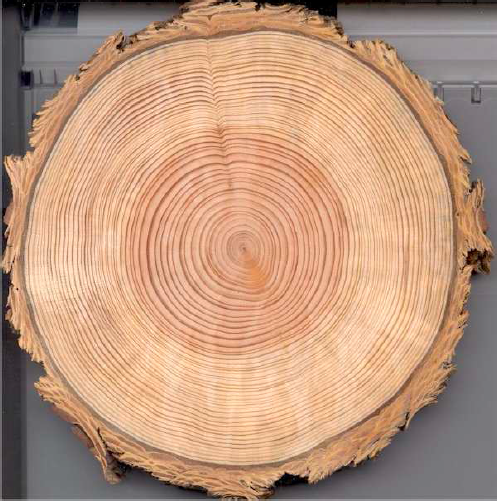
\includegraphics[height=.465\columnwidth]{tree-ring}}
\hfill
\subcaptionbox{Circle view showing six variables over ten time steps as concentric rings. \is{Keim2004} \label{fig:lr-circle-view-2}}{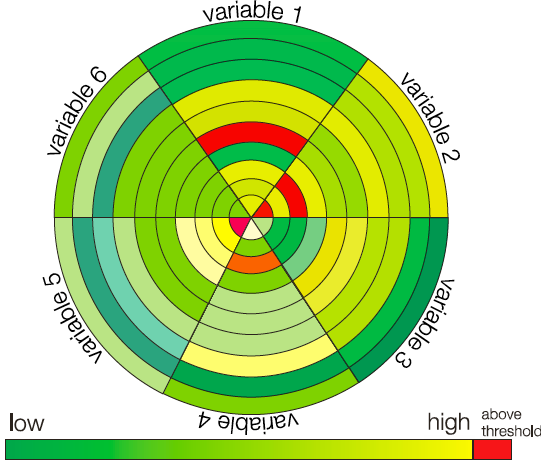
\includegraphics[height=.465\columnwidth]{circle-view}}
\caption{Tree ring. Concentric rings expanding from the center, each indicating a time step.}
\label{fig:lr-circle-view}
\end{figure}

Based on tree-rings, Therón~\cite{Theron2006} develops a technique to show both temporal and hierarchical information. \autoref{fig:lr-tree-ring-time} shows a simple example of such a dataset as tree with five nodes, each is associated with a timestamp. These nodes are assigned to the rings based on their temporal values before being positioned along the ring in such a way that arrows can be drawn from parent nodes to child nodes to reflect the hierarchy (\autoref{fig:lr-tree-ring-tree}).

\begin{figure}[!htb]
\centering
\subcaptionbox{Hierarchy is shown as a tree with temporal values are annotated next to the nodes. \label{fig:lr-tree-ring-time}}[.48\columnwidth]{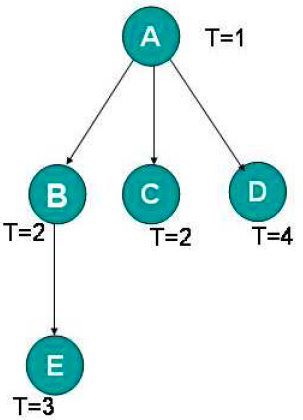
\includegraphics[height=.4\columnwidth]{tree-ring-time}}
\hfill
\subcaptionbox{Hierarchy is shown as a tree embedded on a circle view with rings indicating temporal values. \label{fig:lr-tree-ring-tree}}[.48\columnwidth]{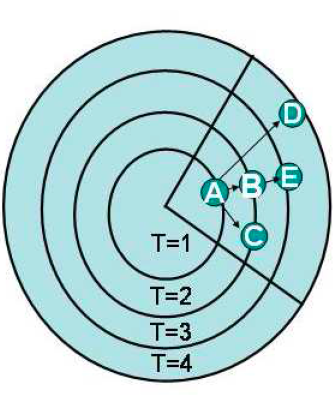
\includegraphics[height=.4\columnwidth]{tree-ring-tree}}
\caption{Visualizing both temporal and hierarchical information using tree rings. \is{Theron2006}}
\end{figure}

\subsection{Calendar}
Another method to represent time is using a \emph{calendar}. A day is usually color coded based on its value to reveal patterns in the data. A calendar visualization allows users to identify patterns at different temporal granularities such as daily, weekly and monthly.  \autoref{fig:lr-calendar} visualizes the daily power consumption over a year with color indicating the result of a clustering algorithm. Several patterns can be observed in this figure. First, the energy consumption is low in the summer and on Fridays. Second, it is even lower at weekends and holidays such as Christmas and New Year. Third, this figure shows the energy consumed in Netherlands, thus some patterns are clear for Dutch people such as on December 5th, employees can leave their office earlier to celebrate Santa Claus.

\begin{figure}[!htb]
	\centering
	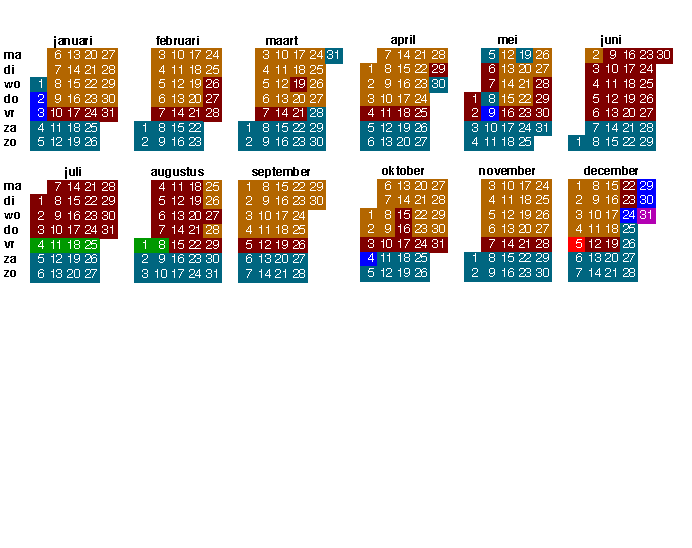
\includegraphics[width=\columnwidth]{calendar}
	\caption{Calendar visualization of a one-year data of daily power consumption. A cell for each day is color coded to reveal data patterns. \is{VanWijk1999}}
	\label{fig:lr-calendar}
\end{figure}

\subsection{Small Multiples}
Another method to depict changes over time is \emph{small multiples} -- a set of miniature visual representations placed next to each other with each showing the visualization at a selected time step~\cite{Tufte1983}. Small multiples provide an overview of the data and allow users to visually compare it at different time points. The concept is general and can be applied to virtually all static visualization techniques because only thumbnails of the visualization for each time step are required. \autoref{fig:lr-small-multiples} shows an example of small multiples of bar charts.

\begin{figure}[!htb]
	\centering
	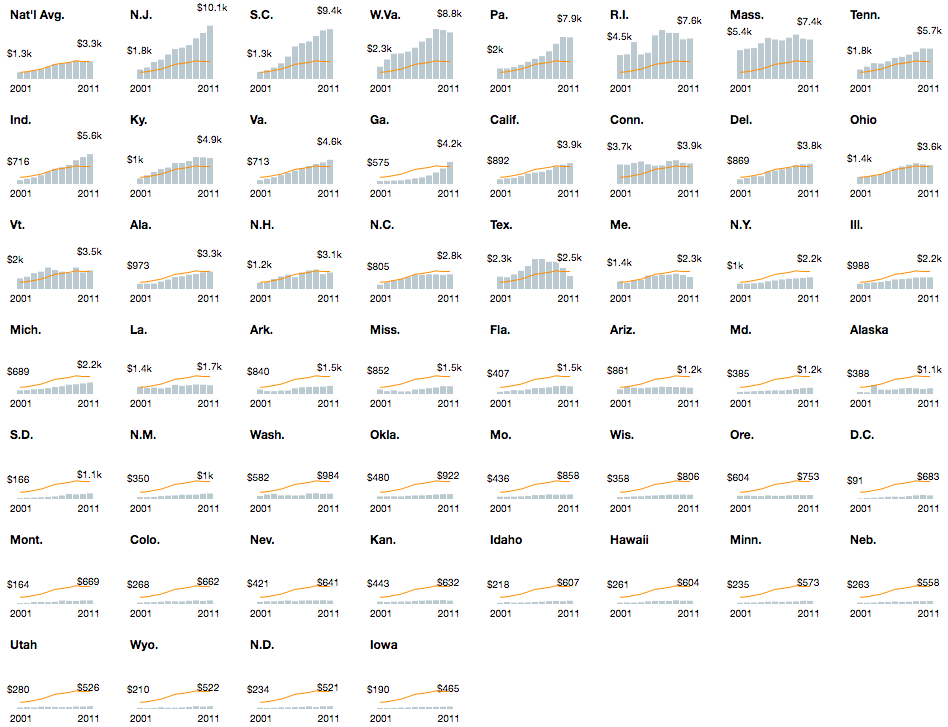
\includegraphics[width=\columnwidth]{small-multiples}
	\caption{Small multiples of bar charts showing average annual Medicare spending on ambulance services per dialysis patient by U.S. state from 2001 to 2011. \is{SmallMultiples2014}}
	\label{fig:lr-small-multiples}
\end{figure}

To facilitate the exploration of relationship in the data at multiple time steps, the miniatures should be interactive and linked together, rather than just static thumbnails. \autoref{fig:lr-small-multiples} shows small interactive bar charts sorted decreasingly by the value spend on the last year. Alternatively, they can be ordered alphabetically by state names to facilitate searching. Standard brushing and linking interaction technique also helps compare the subsets of interest. A limitation of this method is scalability. The number of representable time steps are relatively small because of the thumbnail size.

\subsection{Animation}
Animation is another technique to convey time that can be applied to virtually all static visualization techniques. It relies on human perception in perceiving changes when a visualization smoothly updates from one time step to another. The most notable example is Trendalyzer by Gapminder Foundation~\cite{Gapminder} -- an interactive visualization and presentation tool based on scatter plots. The animation is controlled via a time slider, a play/pause button, and a speed slider. Only a few data items should be animated, and they are often highlighted so that the user can keep track of the changes. Trails may also be displayed to maintain the path of a data item through time. A study by Robertson~et~al.~\cite{Robertson2008} shows that animation is both slower and less accurate than small multiples in conveying trends over time.

\begin{figure}[!htb]
	\centering
	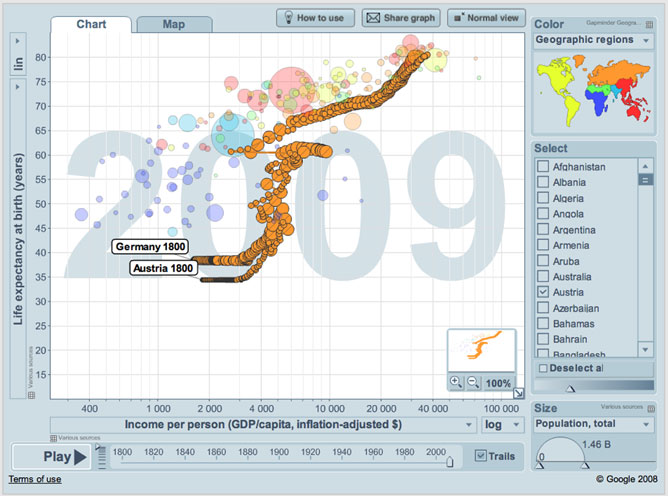
\includegraphics[width=\columnwidth]{animation}
	\caption{Trendalyzer interface. A scatter plot with an animation controller to traverse through time. Additionally, trails are activated for the selected countries, Austria and Germany, which help to preserve the path of a variable in animation. \is{Aigner2011}}
	\label{fig:lr-animation}
\end{figure}

Besides showing trends of time-series data, animation has also been applied in other temporal datasets. Animation is a powerful and appealing technique in presentation of a known story~\cite{Gershon2001}. It helps illustrate computer algorithms step by step and motivate students in approaching complex problems~\cite{Kehoe2001}. Animation also allows reproduction of a data exploration process by interpolating visual parameters of key saved visualization steps~\cite{Ma1999}.

\subsection{Summary}
in this section, we discuss mapping techniqeus ... list all mappings. we contribute novel temporal + sensemaking activities. also a timsets